% Pengaturan ukuran teks dan bentuk halaman dua sisi
\documentclass[12pt]{book}

% Pengaturan ukuran halaman dan margin
\usepackage[a4paper,top=30mm,left=30mm,right=20mm,bottom=25mm]{geometry}

% Pengaturan ukuran spasi
\usepackage[singlespacing]{setspace}

% Pengaturan caption untuk tabel
\usepackage{caption}

% Judul dokumen
\title{Proposal Tugas Akhir ITS}
\author{Aptanagi, Urdhanaka}

% Pengaturan detail pada file PDF
\usepackage[pdfauthor={\@author},bookmarksnumbered,pdfborder={0 0 0}]{hyperref}

% Pengaturan ukuran indentasi
\setlength{\parindent}{2em}

% Package lainnya
\usepackage{changepage}
\usepackage{etoolbox} % Mengubah fungsi default

% Pengaturan jenis karakter
\usepackage[utf8]{inputenc}
\usepackage{url}

\usepackage[style=apa, backend=biber]{biblatex}
\usepackage{xurl}
\usepackage{enumitem} % Pembuatan list
\usepackage{graphicx} % Input gambar
\usepackage{longtable} % Pembuatan tabel
\usepackage[table,xcdraw]{xcolor} % Pewarnaan tabel
\usepackage{eso-pic} % Untuk menggunakan background image di halaman
\usepackage{txfonts} % Font times
\usepackage{changepage} % Pembuatan teks kolom
\usepackage{multicol} % Pembuatan kolom ganda
\usepackage{multirow} % Pembuatan baris ganda
\usepackage{tabularx} % Untuk mengatur kolom, seperti grid pada CSS
\usepackage{wrapfig}
\usepackage{float}

% Pengaturan format daftar isi, daftar gambar, dan daftar tabel
\usepackage[titles]{tocloft}
\setlength{\cftsecindent}{2em}
\setlength{\cftsubsecindent}{2em}
\setlength{\cftbeforechapskip}{1.5ex}
\setlength{\cftbeforesecskip}{1.5ex}
\setlength{\cftbeforetoctitleskip}{0cm}
\setlength{\cftbeforeloftitleskip}{0cm}
\setlength{\cftbeforelottitleskip}{0cm}
\renewcommand{\cfttoctitlefont}{\hfill\Large\bfseries} % command untuk membuat heading bold dan besar
\renewcommand{\cftaftertoctitle}{\hfill}
\renewcommand{\cftloftitlefont}{\hfill\Large\bfseries}
\renewcommand{\cftafterloftitle}{\hfill}
\renewcommand{\cftlottitlefont}{\hfill\Large\bfseries}
\renewcommand{\cftafterlottitle}{\hfill}

% Definisi untuk "Hati ini sengaja dikosongkan"
\patchcmd{\cleardoublepage}{\hbox{}}{
  \thispagestyle{empty}
  \vspace*{\fill}
  \begin{center}\textit{[Halaman ini sengaja dikosongkan]}\end{center}
  \vfill}{}{}

% Pengaturan penomoran halaman
\usepackage{fancyhdr}
\fancyhf{}
\renewcommand{\headrulewidth}{0pt}
\pagestyle{fancy}
\fancyfoot[C,CO]{\thepage}
\patchcmd{\chapter}{plain}{fancy}{}{}
\patchcmd{\chapter}{empty}{plain}{}{}

% Pengaturan format judul bab
\usepackage{titlesec}
\renewcommand{\thesection}{\thechapter.\arabic{section}}
\titleformat{\chapter}[hang]{\centering\bfseries\large}{BAB\ \arabic{chapter}\ }{0ex}{\vspace{0ex}\centering}
\titleformat*{\section}{\large\bfseries}
\titleformat*{\subsection}{\normalsize\bfseries}
\titlespacing{\chapter}{0ex}{0ex}{4ex}
\titlespacing{\section}{0ex}{1ex}{0ex}
\titlespacing{\subsection}{0ex}{0.5ex}{0ex}
\titlespacing{\subsubsection}{0ex}{0.5ex}{0ex}
\setcounter{secnumdepth}{3} % Untuk memberi penomoran pada \subsubsection

\counterwithin{figure}{chapter}
\counterwithin{table}{chapter}

% Mengganti figure dan table menjadi gambar dan tabel
\renewcommand{\figurename}{Gambar}
\renewcommand{\tablename}{Tabel}

% Tambahkan format tanda hubung yang benar di sini
\hyphenation{
  ro-ket
  me-ngem-bang-kan
  per-hi-tu-ngan
}

% Menambahkan resource daftar pustaka
\addbibresource{pustaka/pustaka.bib}

% Isi keseluruhan dokumen
\begin{document}
  % Nomor halaman pembuka dimulai dari sini
  \pagenumbering{roman}

  % Atur ulang penomoran halaman
  \setcounter{page}{1}

  % Sampul Bahasa Indonesia
  \newcommand\covercontents{sampul/konten-id.tex}
  \AddToShipoutPictureBG*{
  \AtPageLowerLeft{
    % Ubah nilai berikut jika posisi horizontal background tidak sesuai
    \hspace{-3.25mm}

    % Ubah nilai berikut jika posisi vertikal background tidak sesuai
    \raisebox{0mm}{
      
\includegraphics[width=\paperwidth,height=\paperheight]{sampul/gambar/sampul-luar-tipis.png}
    }
  }
}

% Menyembunyikan nomor halaman
\thispagestyle{empty}

% Pengaturan margin untuk menyesuaikan konten sampul
\newgeometry{
  top=65mm,
  left=30mm,
  right=30mm,
  bottom=20mm
}

\begin{flushleft}

  % Pemilihan font sans serif
  \sffamily

  % Pemilihan font bold
  \fontseries{bx}
  \selectfont
  \begin{spacing}{1.5}
    \input{\covercontents}
  \end{spacing}

\end{flushleft}

\restoregeometry


  % Lembar pengesahan
  \chapter*{LEMBAR PENGESAHAN}

% Menyembunyikan nomor halaman
\thispagestyle{empty}

\begin{center}
  % Ubah kalimat berikut dengan judul tugas akhir
  \textbf{IMPLEMENTASI \emph{MULTI-TENANCY} UNTUK \emph{PROVISIONING CLUSTER} KUBERNETES}
\end{center}

\begingroup
% Pemilihan font ukuran small
\small

\begin{center}
  % Ubah kalimat berikut dengan pernyataan untuk lembar pengesahan
  \textbf{PROPOSAL TUGAS AKHIR} \\
  Diajukan untuk memenuhi salah satu syarat memperoleh gelar
  Sarjana Komputer pada
  Program Studi S-1 Teknik Informatika \\
  Departemen Teknik Informatika \\
  Fakultas Teknologi Elektro dan Informatika Cerdas \\
  Institut Teknologi Sepuluh Nopember
\end{center}

\begin{center}
  % Ubah kalimat berikut dengan nama dan NRP mahasiswa
  Oleh: \textbf{Urdhanaka Aptanagi} \\
  NRP. 5025211123
\end{center}

\begin{center}
  Disetujui Oleh:
\end{center}

\vspace{10ex}

\begingroup
% Menghilangkan padding
\setlength{\tabcolsep}{0pt}

\noindent
\begin{tabularx}{\textwidth}{X c}
  % Ubah kalimat-kalimat berikut dengan nama dan NIP dosen pembimbing pertama
        &                 \\
  Royyana Muslim Ijtihadie, S.Kom. ,M.Kom., Ph.D      &                 \\
  NIP: 19770824 200604 1 001                          & (Pembimbing)    \\
                                                      &                 \\
                                                      &                 \\
                                                      &                 \\
  % Ubah kalimat-kalimat berikut dengan nama dan NIP dosen pembimbing kedua
  Ary Mazharuddin Shiddiqi, S.Kom., M.Comp.Sc., Ph.D  &                 \\
  NIP: 19810620 200501 1 003                          & (Ko-Pembimbing) \\
\end{tabularx}
\endgroup

\vspace{\fill}

\begin{center}
  Mengetahui,\\
  % Ubah kalimat berikut dengan nama departemen
  Kepala Departemen Teknik Informatika FTEIC-ITS\\
  \vspace{10ex}
  % Ubah kalimat berikut dengan jabatan kepala departemen
  \underline{Nikola Tesla, S.T., M.T. }\\
  NIP 18560710 194301 1 001\\
  \vspace{10ex}
  % Ubah text dibawah menjadi tempat dan tanggal
  \textbf{SURABAYA} \\
  \textbf{Mei, 2024}
\end{center}
\endgroup

  \cleardoublepage

  % Abstrak
  \chapter*{ABSTRAK}
\begin{center}
  \large
  \textbf{IMPLEMENTASI \emph{MULTI-TENANCY} UNTUK \emph{PROVISIONING CLUSTER} KUBERNETES}
\end{center}
\addcontentsline{toc}{chapter}{ABSTRAK}
% Menyembunyikan nomor halaman
\thispagestyle{empty}

\begin{flushleft}
  \setlength{\tabcolsep}{0pt}
  \bfseries
  \begin{tabular}{ll@{\hspace{6pt}}l}
  Nama Mahasiswa / NRP&:& Urdhanaka Aptanagi / 5025211123\\
  Departemen&:& Teknik Informatika FTEIC - ITS\\
  Dosen Pembimbing&:& 1. Nikola Tesla, S.T., M.T.\\
  & & 2. Wernher von Braun, S.T., M.T.\\
  \end{tabular}
  \vspace{4ex}
\end{flushleft}
\textbf{Abstrak}

% Isi Abstrak
Sistem terdistribusi merupakan salah satu cara untuk meningkatkan kinerja
dan keandalan sebuah sistem. Sebuah \emph{tools} yang sering digunakan dalam sistem
terdistribusi adalah Kubernetes.

\vspace{2ex}
\noindent
\textbf{Kata Kunci: \emph{multi-tenancy, virtual cluster, kubernetes}}

  \cleardoublepage

  \chapter*{ABSTRACT}
\begin{center}
  \large
  \textbf{\emph{ANTI-GRAVITY} BASED ENERGY CALCULATION ON OUTER SPACE ROCKETS}
\end{center}
% Menyembunyikan nomor halaman
\thispagestyle{empty}

\begin{flushleft}
  \setlength{\tabcolsep}{0pt}
  \bfseries
  \begin{tabular}{lc@{\hspace{6pt}}l}
  Student Name / NRP&: &Urdhanaka Aptanagi / 5025211123\\
  Department&: &Informatics Engineering FTD - ITS\\
  Advisor&: &1. Nikola Tesla, S.T., M.T.\\
  & & 2. Wernher von Braun, S.T., M.T.\\
  \end{tabular}
  \vspace{4ex}
\end{flushleft}
\textbf{Abstract}

% Isi Abstrak
test. \lipsum[1]

\vspace{2ex}
\noindent
\textbf{Keywords: \emph{multi-tenancy, virtual cluster, kubernetes}}

  \cleardoublepage

  \begin{spacing}{1}
    % Daftar isi
    \renewcommand*\contentsname{DAFTAR ISI}
    \addcontentsline{toc}{chapter}{\contentsname}
    \tableofcontents
    \cleardoublepage

    % Daftar gambar
    % \renewcommand*\listfigurename{DAFTAR GAMBAR}
    % \addcontentsline{toc}{chapter}{\listfigurename}
    % \listoffigures
    % \cleardoublepage

    % Daftar tabel
    \renewcommand*\listtablename{DAFTAR TABEL}
    \addcontentsline{toc}{chapter}{\listtablename}
    \listoftables
    \cleardoublepage
  \end{spacing}

  % Nomor halaman isi dimulai dari sini
  \pagenumbering{arabic}

  % Konten pendahuluan
  \chapter{PENDAHULUAN}

\section{Latar Belakang}

Internet merupakan salah satu inovasi yang mengubah dunia. Internet
memungkinkan penggunanya untuk berkomunikasi, berbagi informasi, dan
mengakses berbagai layanan. Salah satu bentuk layanan tersebut adalah
layanan komputasi dimana pengguna dapat menggunakan sumber daya komputasi
yang telah disediakan sehingga pengguna tidak perlu melakukan komputasi
di perangkat mereka sendiri. Hal tersebut memungkinkan pengguna untuk
melakukan komputasi yang berat tanpa harus memiliki perangkat yang
memadai.

Pengelolaan sumber daya komputasi memerlukan manajemen yang
baik agar sumber daya tersebut dapat digunakan secara efisien dan sesuai
dengan kebutuhan pengguna. Untuk mengelola sumber daya komputasi tersebut,
salah satu \emph{tools} yang dapat digunakan adalah Kubernetes. Kubernetes
adalah sebuah sistem manajemen \emph{container} sumber terbuka.

Namun, penggunaan Kubernetes secara \emph{default} bukan berupa \emph{multi-tenant}.
Semua \emph{pods} yang merupakan unit terkecil di dalam Kubernetes dapat berinteraksi
satu sama lain dan semua \emph{network traffic} tidak terenkripsi \parencite{kubernetes-website-multi-tenancy}.
Hal tersebut dapat menimbulkan masalah karena pengguna yang satu dapat
melihat data dari pengguna yang lain. Oleh karena itu, diperlukan
implementasi \emph{multi-tenancy} pada Kubernetes jika sebuah kluster Kubernetes
akan digunakan oleh lebih dari satu pengguna.

Pada penelitian ini akan dibahas mengenai implementasi \emph{multi-tenancy}
pada Kubernetes. Implementasi tersebut diharapkan membuat kluster
Kubernetes dapat digunakan oleh beberapa pengguna sekaligus.

\section{Rumusan Masalah}

Berdasarkan hal yang telah dipaparkan di latar belakang, rumusan masalah
yang diangkat dalam Tugas Akhir ini adalah sebagai berikut:
\begin{enumerate}
  \vspace{-0.3cm}\item{Bagaimana cara mengimplementasikan \emph{multi-tenancy} pada kluster Kubernetes?}
  \vspace{-0.3cm}\item{Apa perbedaan implementasi \emph{multi-tenancy} yang dapat digunakan pada kluster Kubernetes?}
\end{enumerate}

\section{Batasan Masalah atau Ruang Lingkup}

Batasan masalah atau ruang lingkup dari penelitian ini adalah sebagai berikut:
\begin{enumerate}
  \vspace{-0.3cm}\item{asdasdad}
\end{enumerate}

\section{Tujuan}

Tujuan dari penelitian ini adalah mengimplementasikan \emph{multi-tenancy}
pada kluster Kubernetes yang dapat digunakan.

\section{Manfaat}

Manfaat dari penelitian ini adalah 

  \cleardoublepage

  % Konten tinjauan pustaka
  \chapter{TINJAUAN PUSTAKA}

% Ubah konten-konten berikut sesuai dengan isi dari tinjauan pustaka
\section{Hasil penelitian/perancangan terdahulu}
\lipsum[3]

\section{Teori/Konsep Dasar}

\subsection{Hukum Newton}

% Contoh penggunaan referensi dari pustaka
Newton pernah merumuskan \parencite{Newton1687} bahwa \lipsum[8]
% Contoh penggunaan referensi dari persamaan
Kemudian menjadi persamaan seperti pada persamaan \ref{eq:FirstLaw}.

% Contoh pembuatan persamaan
\begin{equation}
  % Label referensi dari persamaan yang dibuat
  \label{eq:FirstLaw}
  % Baris kode persamaan yang dibuat
  \sum \mathbf{F} = 0\; \Leftrightarrow\; \frac{\mathrm{d} \mathbf{v} }{\mathrm{d}t} = 0.
\end{equation}

\lipsum[9]

\subsection{Anti Gravitasi}

\lipsum[10]

  \cleardoublepage

  % Konten metodologi
  \chapter{METODOLOGI}

% Ubah konten-konten berikut sesuai dengan isi dari metodologi

\section{Metode yang digunakan}

\lipsum[11]

% Contoh input gambar dengan format *.jpg
\begin{figure} [H] \centering
  % Nama dari file gambar yang diinputkan
  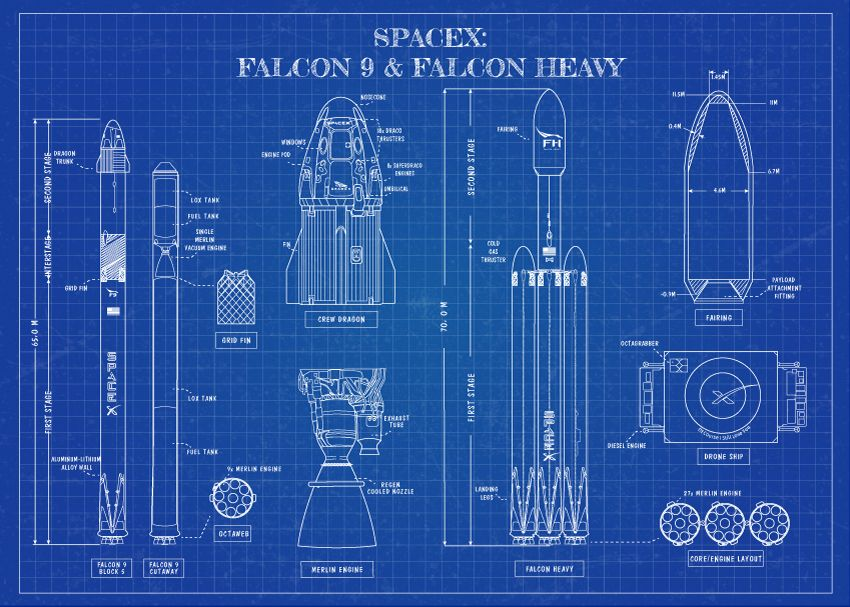
\includegraphics[scale=0.45]{gambar/blueprint.jpg}
  % Keterangan gambar yang diinputkan
  \caption{\emph{Blueprint} roket yang akan diuji coba}
  % Label referensi dari gambar yang diinputkan
  \label{fig:Blueprint}
\end{figure}

% Contoh penggunaan referensi dari gambar yang diinputkan
Pada \emph{blueprint} yang tertera di Gambar \ref{fig:Blueprint}. Pada \parencite{6830928}

\section{Bahan dan peralatan yang digunakan}

\lipsum[13]

  \cleardoublepage

  \chapter{JADWAL PENELITIAN}

% Ubah tabel berikut sesuai dengan isi dari rencana kerja
\newcommand{\w}{}
\newcommand{\G}{\cellcolor{gray}}
\begin{table}[H]
  \captionof{table}{Tabel timeline}
  \label{tbl:timeline}
  \begin{tabular}{|p{3.5cm}|c|c|c|c|c|c|c|c|c|c|c|c|c|c|c|c|}

    \hline
    \multirow{2}{*}{Kegiatan} & \multicolumn{16}{|c|}{Minggu}                                                                       \\
    \cline{2-17}              &
    1                         & 2                             & 3  & 4  & 5  & 6  & 7  & 8  & 9  & 10 & 11 & 12 & 13 & 14 & 15 & 16 \\
    \hline

    % Gunakan \G untuk mengisi sel dan \w untuk mengosongkan sel
    Pengambilan data          &
    \G                        & \G                            & \G & \G & \w & \w & \w & \w & \w & \w & \w & \w & \w & \w & \w & \w \\
    \hline

    Pengolahan data           &
    \w                        & \w                            & \w & \w & \G & \G & \G & \G & \w & \w & \w & \w & \w & \w & \w & \w \\
    \hline

    Analisa data              &
    \w                        & \w                            & \w & \w & \w & \w & \w & \w & \G & \G & \G & \G & \w & \w & \w & \w \\
    \hline

    Evaluasi penelitian       &
    \w                        & \w                            & \w & \w & \w & \w & \w & \w & \w & \w & \w & \w & \G & \G & \G & \G \\
    \hline
  \end{tabular}
\end{table}

Pada \emph{timeline} yang tertera di Tabel \ref{tbl:timeline}

  \cleardoublepage

  % Daftar pustaka
  \chapter*{DAFTAR PUSTAKA}
  \addcontentsline{toc}{chapter}{DAFTAR PUSTAKA}
  \renewcommand\refname{}
  \vspace{2ex}
  \renewcommand{\bibname}{}
  \begingroup
    \def\chapter*#1{}
    \printbibliography
  \endgroup

\end{document}
